% !TEX root = ../../../main.tex
% 来源：中学数学实验教材·第三册（高中数学）
% 章节：三角函数的图象和性质 / 正弦函数的图象和性质
% 原始文件：7.tex，行 163-224
% 类型：tikz
% ---
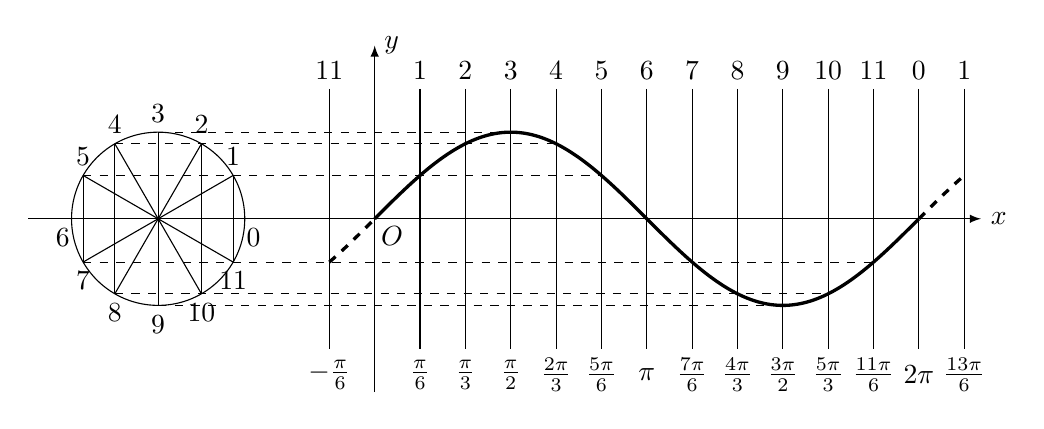
\begin{tikzpicture}[>=latex,scale=1.1]

\draw[->] (-4,0)--(7,0)node[right]{$x$};
\draw [->](0,-2)--(0,2)node[right]{$y$};
\draw (-2.5,0) circle (1);

\draw[domain=0 : pi*2,  samples=1000, very thick] plot(\x, {sin(\x r)});

\foreach \x in {1,2,...,11}
{
    \draw (\x*pi/6,1.5)node[above]{\x}--(\x*pi/6,-1.5);
}

\foreach \x in {1,2,...,5}
{
    \draw (-2.5,0)--+ (\x*30:1)node[above]{\x};
}
\foreach \x in {7,8,...,11}
{
    \draw (-2.5,0)--+ (\x*30:1)node[below]{\x};
}



\draw (-2.5+.5, .5*1.732)--(-2.5+.5, -.5*1.732);
\draw (-2.5-.5, .5*1.732)--(-2.5-.5, -.5*1.732);
\draw (-2.5-.5*1.732, .5)--(-2.5-.5*1.732, -.5);
\draw (-2.5+.5*1.732, .5)--(-2.5+.5*1.732, -.5);
\draw [dashed] (-2.5-.5, .5*1.732)--(2*pi/3, .5*1.732);
\draw [dashed] (-2.5-.5*1.732, .5)--(5*pi/6, .5);
\draw [dashed] (-2.5-.5, -.5*1.732)--(5*pi/3, -.5*1.732);
\draw [dashed] (-2.5-.5*1.732, -.5)--(11*pi/6, -.5);

\draw[dashed] (-2.5, 1)--(pi/2, 1);
\draw [dashed](-2.5, -1)--(1.5*pi, -1);
\node at (-1*pi/6,-1.8){$-\frac{\pi}{6}$};
\node at (13*pi/6,-1.8){$\frac{13\pi}{6}$};
\node at (1*pi/6,-1.8){$\frac{\pi}{6}$};
\node at (2*pi/6,-1.8){$\frac{\pi}{3}$};
\node at (3*pi/6,-1.8){$\frac{\pi}{2}$};
\node at (4*pi/6,-1.8){$\frac{2\pi}{3}$};
\node at (5*pi/6,-1.8){$\frac{5\pi}{6}$};
\node at (6*pi/6,-1.8){$\pi$};
\node at (7*pi/6,-1.8){$\frac{7\pi}{6}$};
\node at (8*pi/6,-1.8){$\frac{4\pi}{3}$};
\node at (9*pi/6,-1.8){$\frac{3\pi}{2}$};
\node at (10*pi/6,-1.8){$\frac{5\pi}{3}$};
\node at (11*pi/6,-1.8){$\frac{11\pi}{6}$};
\node at (12*pi/6,-1.8){$2\pi$};

\draw (-pi/6,1.5)node[above]{11}--(-pi/6,-1.5);
\draw (2*pi,1.5)node[above]{0}--(2*pi,-1.5);
\draw (13*pi/6,1.5)node[above]{1}--(13*pi/6,-1.5);

\draw[domain=-pi/6: 0,  samples=100, very thick, dashed] plot(\x, {sin(\x r)});
\draw[domain=pi*2:13*pi/6,  samples=100, very thick, dashed] plot(\x, {sin(\x r)});

\node at (-1.4, 0)[below]{0};
\node at (-3.6, 0)[below]{6};

\node at (.2,-.2){$O$};
\end{tikzpicture}
